\subsection{Analysis of the plant}
\label{sec:plant}
The transfer function of the plant is
\begin{equation}
    G(s) = \frac{s+20}{s\qty(s^2 + 24s + 144)}
    \label{eq:plant}
\end{equation}
Clearly, the system has two poles at $s = -12$ and one pole at the origin. There is one zero located at $s = -20$ (all on the real axis). A pole-zero map of the system is shown in \cref{fig:cont_plant_pzmap}. 
\begin{figure}[ht]
    \centering
    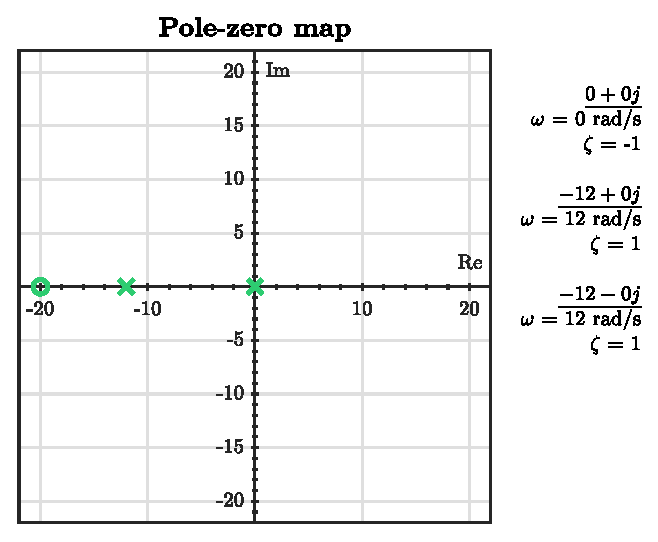
\includegraphics[]{media/q1/cont_plant_pzmap.eps}
    \caption{Pole-zero map of the continuous-time plant model. Clearly, the plant has only real, stable poles and zeros.}
    \label{fig:cont_plant_pzmap}
\end{figure}
From inspection of the poles and zeros, it can be concluded that the plant is \nth{3}-order, minimum phase and open-loop stable. Furthermore, because of the pole at $s = 0$, this is a so-called Type-I system. This means that the system is able to track a step reference with perfect steady-state accuracy. Looking at the frequency response function associated with \cref{eq:plant} shown in \cref{fig:cont_plant_bode}, a few additional remarks can be made:
\begin{itemize}
    \item Because the system is Type-I, it approaches $j\omega = 0$ with a slope of \SI{-20}{\decibel\per dec}.
    \item The stability margins of the system are ample: the phase margin is \ang{89.1} and the gain margin infinitely large since the system never crosses (although barely) the \ang{-180}-line. The system is therefore \textit{structurally} stable, i.e. the gain can be increased arbitrarily without causing the poles to venture into the right-half plane.
    \item Overall, the plant shows moderate gains around for low-frequencies and very strong attenuation of frequencies higher than those associated with the double pole at \SI{12}{\radian\per\second}.
\end{itemize}

\begin{figure}[ht]
    \centering
    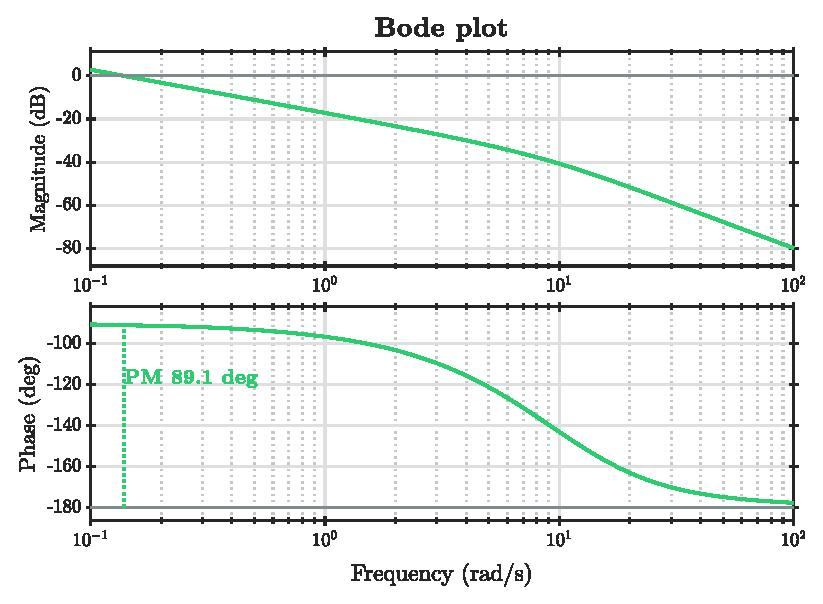
\includegraphics[]{media/q1/cont_plant_bode.eps}
    \caption{Bode plot of the plant. The stability margins are indicated on the plot (the phase margin is \ang{89.1}, the gain margin is infinite).}
    \label{fig:cont_plant_bode}
\end{figure}

\subsection{Set-point tracking\textnormal{\phantom{xxx}(Question 1)}}
\label{sec:continuoustracking}
First, a PID-controller has to be designed for reference-tracking. The following constraints are imposed on the design:
\begin{itemize}
    \item Minimal settling-time
    \item The response overshoot shall not exceed 5\%
    \item No steady-state error
\end{itemize}

\paragraph{Controller structure}
Because the system is Type-I, integral action will not be necessary to avoid steady-state tracking errors. Although the stability margins are very generous, adequate performance may be achieved purely by proportional control. However, due to the strict overshoot requirements and the desire to reduce the settling-time to an absolute minimum, more damping will likely be required in the form of one or two D-terms, resulting in a PD(D)-type controller.

\paragraph{Frequency-domain requirements}
The formerly stated requirements are specified in the time-domain. Because the controller design will be achieved by shaping the loop transfer function, it makes sense to translate these requirements to an (approximate) frequency-domain counterpart. Because analytical results only exist for \nth{2}-order plants, these results will only serve as an approximate target value. Some iteration using a simulation of the closed-loop step response will be inevitable to fine-tune the controller design.

As specified by \textcite{nise}, the following relations hold for a \nth{2}-order plant. First of all, the relation between the bandwidth of the closed-loop system and its settling time is:
\begin{equation}
    \omega_{BW} = \frac{4}{T_s\zeta}\sqrt{\qty(1 - 2\zeta^2)+\sqrt{4
    \zeta^4-4\zeta^2+2}}
    \label{eq:damping}
\end{equation}
Hence, to minimize the settling time one preferably has a damping ration $\zeta$ close to unity and maximise the $\omega_\text{BW}$, which in turn means that the cross-over frequency of the loop transfer function should be as large as possible. Furthermore, the overshoot of the system can be related to the damping ratio as follows:
\begin{equation}
\%\text{OS} = 100\times \exp(-\frac{\zeta \pi}{\sqrt{1-\zeta^2}})
\label{eq:overshoot}    
\end{equation}
This equation suggests that for an overshoot of 5\%, one should aim for $\zeta \approx 0.69$.
Since $\zeta$ is still not directly visible on the loop transfer Bode plot, there also exists a relation between the damping ratio and the phase margin $\phi_m$:
\begin{equation}
\phi_m = \tan[-1](\frac{2\zeta}{\sqrt{-2\zeta^2 + 1 + \sqrt{1 + 4\zeta^4}}})
\label{eq:settlingtime}    
\end{equation}
Based on the required $\zeta$, this yields a target for the phase margin of ca. \ang{64.2}.

\paragraph{Loop shaping}
The computed target phase margin suggests to start with pure proportional control and increase $K_p$ until the phase margin has decreased from \ang{89.1} to \ang{64.6}. \Cref{fig:cont_plant_bode} hints that the new crossover frequency should then be at \SI{4}{\radian\per\second}, which means the gain can be increased by \SI{29.9}{\decibel}. This simple step already results in a dramatic increase in the settling time from \SI{32.7}{\second} (no compensation) to \SI{1.04}{\second}. 

The overshoot for this controller is only 4.7\%, which is not quite limiting. As such, there is some more room to increase the gain further to 31.7, which results in a very marginal reduction of the settling time. Now, the limit of simple proportional control has been attained: in order to speed the response up even further, more damping (i.e. phase lead) must be added at the appropriate frequencies in order to observe the overshoot limit.

A realizable PD-controller has the following transfer function:
\begin{equation}
K_p \qty(1 + \frac{sT_d}{1 + sT_d/N}) = K_p\frac{1 + T_d(N+1)s/N}{1 + sT_d/N}
\label{eq:leadcomp}
\end{equation}
which is essentially the same as a lead-compensator with a pole far into the left-half plane ($N \gg 1$). The choice of $N$ determines the second corner frequency and is dependent on the physical implementation of the system and the actuators, since it will determine noise amplification and the initial jump in the controller effort. \textcite{keviczky} recommend this value between 4 and 6 during controller design, after which it can be retuned after testing with the physical plant. Hence, for the controller design, a value of $N=5$ was chosen. The choice of $N$ places an irrevocable limit on the maximum attainable phase contribution by the PI controller, as given by the following equation\footnote{The relations from \textcite{ogata} are based on a different parameterization of the compensator, but they are equivalent to those mentioned in this report.}: \cite{ogata}
\begin{equation}
\phi_\text{max} = \sin[-1](\frac{N}{N + 2}) \approx \ang{45}
\label{eq:maxphi}
\end{equation}
As mentioned before, the maximum phase contribution of the lead contribution occurs at the geometric mean of the pole and zero frequencie: \cite{ogata}
\begin{equation}
    \omega_{\phi_\text{max}} = \frac{N}{T_d\sqrt{N+1}}
    \label{eq:omegamaxphi}
\end{equation}
Using \crefrange{eq:maxphi}{eq:omegamaxphi}, the maximum phase contribution was placed at the highest frequency where the plant could still have the target phase margin of \ang{64.4} (i.e. the frequency at which the plant has a phase of $\ang{180} - \ang{64.4}  - \ang{45}$). This is shown as iteration \#3 in \cref{tab:loopshaping1}. In order to obtain the desired performance, the proportional gain $K_p$ must be adjusted accordingly. The result is iteration \#4 in \cref{tab:loopshaping1}; the settling time shows a substantial reduction of \%65 to \SI{0.39}{\second}. Finally, the controller was tuned a little more: in order to achieve minimal settling time, the response must be well-damped as illustrated by \cref{eq:settlingtime}. The controller was therefore retuned to have a higher phase margin (\ang{70}) --- from \cref{fig:cont_controllers_step} it is clear that this iteration has much better damping and a better settling time.
\begin{figure}
    \centering
    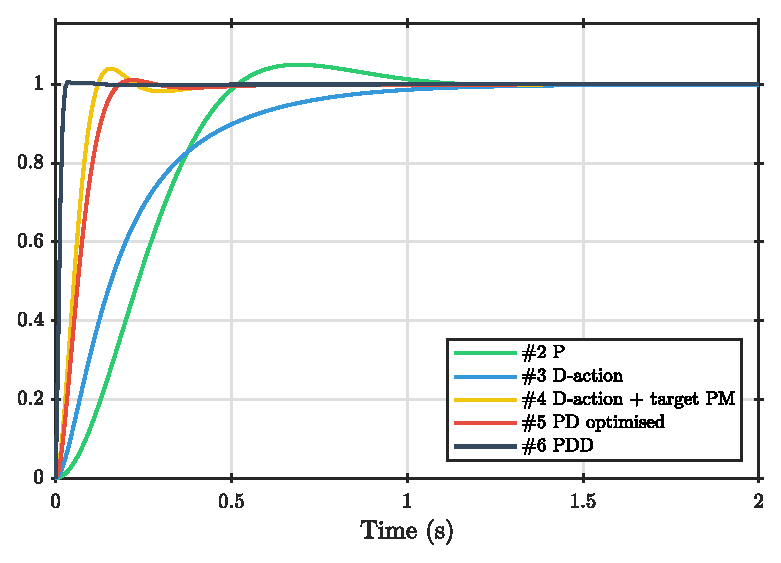
\includegraphics[]{media/q1/pd_controllers_step.eps}
    \caption{}
    \label{fig:cont_controllers_step}
\end{figure}
At this point, the limits of the PD-controller architecture are reached, due to the limited phase contribution given by \cref{eq:maxphi}, sufficient phase margin can only be guaranteed up to a certain frequency. 

Using yet another D-term the phase contribution can be increased even more; the result is a PDD-controller:
\begin{equation}
K_p \qty(1 + \frac{sT_{d_1}}{1 + sT_{d_1}/N})\qty(1 + \frac{sT_{d_2}}{1 + sT_{d_2}/N})
\label{eq:pdd}
\end{equation}
The idea behind the tuning process of these terms was to extend the region with sufficient phase towards higher frequencies without creating excessive `bumps' in the phase curve to obtain an even response. To do so, one lead compensator was placed to have its $\phi_\text{max}$ at about the same frequency as the previous one, while the other one was placed at a frequency about five times higher. The resulting phase and magnitude curves are, together with the previous iterations, displayed in \cref{fig:cont_controllers_bode}. Again, to achieve sufficient damping, the proportional gain was adjusted accordingly for a similar phase margin as iteration \#5, ca. \ang{71}. This final iteration results in a tenfold reduction of the settling time to \SI{0.0251}{\second}.
\begin{figure}[ht]
    \centering
    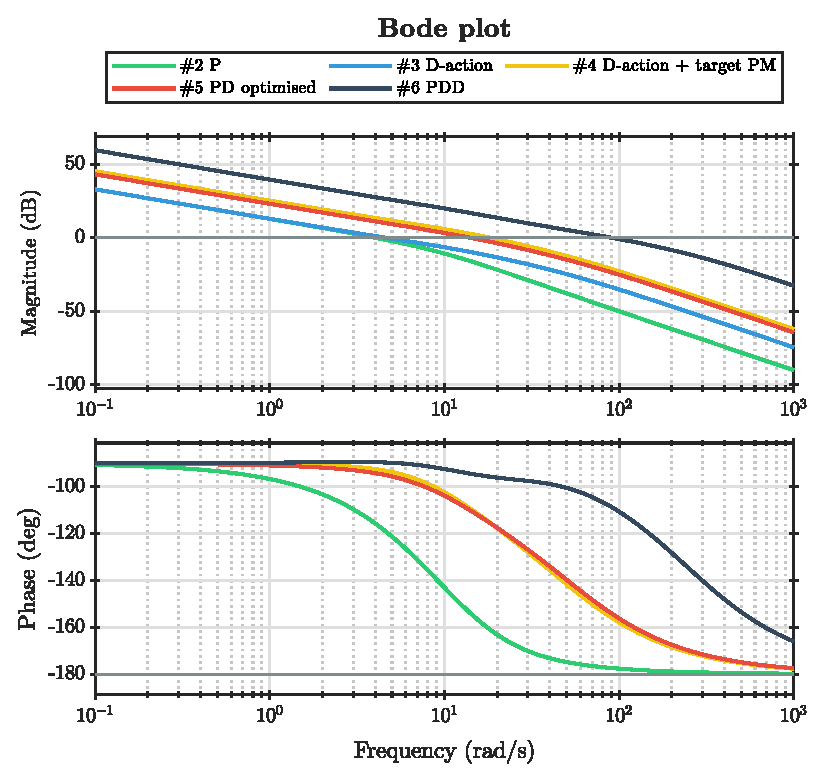
\includegraphics[]{media/q1/pd_controllers_bode.eps}
    \caption{}
    \label{fig:cont_controllers_bode}
\end{figure}
The final PDD controller is then:
$$ 
\begin{aligned}
C(s) &= 675.84\qty(1 + \frac{0.1021s}{1 + s0.1021/5})
            \qty(1 + \frac{0.0204s}{1 + s0.0204/5})\\
     &= \frac{50.69 s^2 + 2483 s + 16896}{0.002083 s^2 + 0.6124 s + 25}
\end{aligned}
$$
\begin{table}[ht]
    \centering
    \caption{Overview of the loop shaping process of the reference tracking controller.}
    \label{tab:loopshaping1}
    \begin{tabular}{ccccccc}
        \toprule
            \# & $K_p$ & $T_{d_1}$ & $T_{d_2}$ & $\phi_m$ (deg) & \%OS & $T_s (\si{\second})$ \\
        \midrule
            0 & 1 & 0 & 0 & 89.1 &  0 & 32.7\\ 
            1 & 31.14 &        0 &        0 &  64.6 &   4.7 &  1.04\\ 
            2 & 31.71 &        0 &        0 &  64.2 &     5 &  1.03\\ 
            3 & 31.71 &    0.112 &        0 &  86.8 &     0 &  1.08\\ 
            4 & 130.8 &    0.112 &        0 &  64.7 &     4 & 0.387\\ 
            5 & 102.4 &    0.102 &        0 &    70 &   1.1 & 0.233\\ 
            6 & 675.8 &    0.102 &   0.0204 &  71.3 &  0.71 & 0.0267\\ 
        \bottomrule
    \end{tabular}
\end{table}

\subsection{Disturbance rejection\textnormal{\phantom{xxx}(Question 2)}}
\label{sec:continuousdisturbance}
In this section, another contoller will be designed specifically for the rejection of a load disturbance $q$ that acts on the control input in the form of a step input. The following requirements are to be fullfilled:
\begin{itemize}
    \item Minimal amplitude of the output as a result of the disturbance.
    \item Minimal duration of the disturbance.
    \item The disturbance shall cause no offset in the response.
\end{itemize}
\paragraph{Controller structure}
The closed-loop transfer function from the load disturbance $q$ to the output $y$ is straightforward to determine:
\begin{equation}
    G_q(s) = \frac{G(s)}{1 + G(s)K(s)} = G(s)S(s)\qq{with}S = \frac{1}{1 + G(s)K(s)}
    \label{eq:disttf}
\end{equation}
where $S(s)$ is the so-called sensitivity transfer function of the closed-loop. Clearly, the sensitivity function will have the poles of the loop transfer function as zeros. \Cref{sec:plant} already mentions that the system is Type-I. Therefore, the sensitivity function must have a \textit{zero} at $s = 0$. As such, in the transfer function $G_d(s)$ the zero from $S$ and the pole from $G_d$ cancel. In order to meet the requirements and have no steady-state offset in the response due to the load disturbance, the final value theorem states that $\lim_{s\to 0} sG_d(s)\frac{1}{s}$. As such, $G_d(s)$ must have a zero at $s = 0$ (which of course should not be cancelled). This can be achieved by placing an extra pole in the controller at $s = 0$; in other words: integral action will be instrumental to eliminate steady-state offset as a result of the load disturbance. Hence, the controller will be of the type PI(DD).

\paragraph{Frequency-domain requirements}
Ideally, the transfer function from the disturbance $q$ to the output $y$ is no-pass (i.e. none of the frequency components in the disturbance persist to the output). Of course, this is not achievable. However, from inspection of \cref{eq:disttf} it is clear that for frequencies where the loop gain $\abs{G(s)K(s)}$ is high will $G_d(s)$ will show proper damping. Hence, high proportional gain and lag compensation (i.e. high gain contribution at lower frequencies) will decrease the settling time of the output after the introduction of the step load disturbance. The plant itself is low-pass with a very low crossover frequency; hence one can expected that high controller gain will be required to reject the disturbance quickly. Besides, the aforementioned requirements will likely contradict with those of the previous controller: where for the tracking case a generous phase margin reduced the settling time, higher damping in the case of disturbance rejection will jeopardise the controller's ability to amplify frequency components to a sufficient extent which in turn would mitigate the effect of the load disturbance on the output.

\paragraph{Loop shaping}
It is already known that a PI-controller structure will be inevitable to obey the imposed constraints. As such, the limits of this controller type will be explored first after which the potential extension to a PID(D) type controller can be investigated. The PI-controller has the transfer function
\begin{equation}
    K_p\qty(1 + \frac{1}{T_is})
\end{equation}
which has a pole at $s = 0$ and a zero at $s = -1/T_i$. The zero determines the second corner frequency of the controller, and therefore up to which frequency the amplification occurs. Simultaneously, the PI controller will introduce a destabilising phase lag for lower frequencies, also determined by the position of this zero.

Because the proportional gain $K_p$ does not affect the phase curve of the system, the maximum attainable phase margin (i.e. where the phase curve is maximal) is purely determined by the choice of $T_i$. A higher phase margin gives better damping of oscillatory respones but also means that $T_i$ must be higher, which decreases the amplification of the lower frequencies with a deterioration of the settling time as a result (the slower frequencies will take longer to be rejected by the system). Oscillations in the response may on the other hand also slow down the time it takes for the output to return to zero, so a compromise has to be found. \Cref{fig:pm_comparison} shows a comparison of three values for the phase margin: for each of these, $T_i$ was tuned to make sure that the maximum attainable phase margin would be equal to a set value (\ang{35}, \ang{41} and \ang{45}), after which $K_p$ was tuned to set the crossover frequency at the correct value. Clearly, the settling time is lowest for $\phi_m = \ang{40}$, so this value was used as an approximate tuning value for $T_i$. 
\begin{figure}
    \centering
    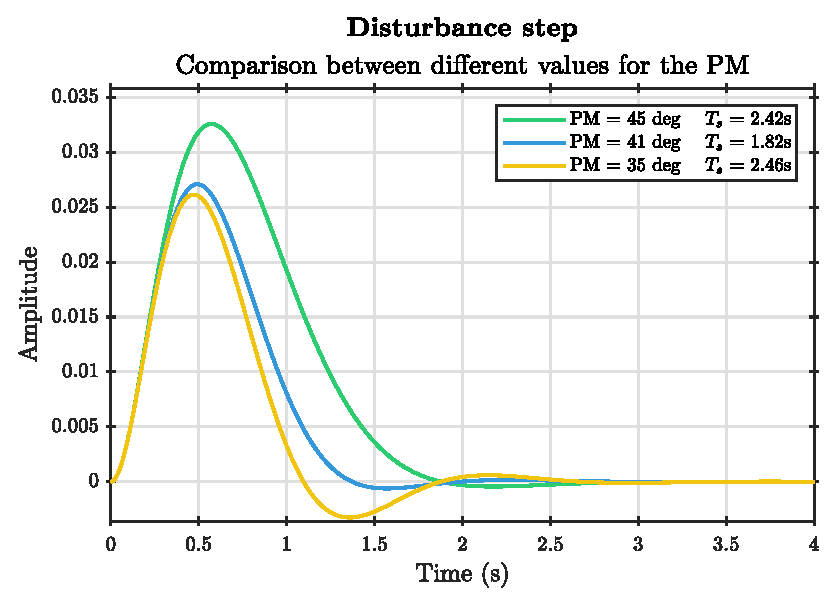
\includegraphics[]{media/q2/pi_pm_comparison.eps}
    \caption{}
    \label{fig:pm_comparison}
\end{figure}

It has to be noted that the two first requirements are conflicting, since both the peak amplitude and the settling time must be minimised, without a quantifiable priority of one over the other. Indeed, in \cref{fig:pm_comparison} one can see that for $\phi_m = \ang{35}$, the peak value is slightly lower. However, because the relative difference in the peak value is relatively low compared to the difference in settling time, $\phi_m = \ang{40}$ is said to show the `better' performance.

At this point, no better performance (in terms of settling time) can be achieved by using the PI controller structure: to lower the settling time $T_i$ must be decreased to amplify the lower frequencies to a greater extent. However, this creates two issues: firstly, the phase curve will at some point cross the \ang{-180} line, which will render the system immediately unstable: the gain will cross-over at a higher frequency. Decreasing the gain is not an option since it will yield a dramatic increase of the peak amplitude. Secondly, as illustrated by \cref{fig:pm_comparison} the smaller phase margin results in badly damped oscillatory artefacts in the response even before the point of instability is reached. Therefore, one must resort to D-action to add phase advance at these higher frequencies to keep sufficient phase margin and prevent the phase from crossing over. As in \cref{sec:continuoustracking}, a realizable D-term as described by \cref{eq:leadcomp} will be used with $N = 5$. 

\sisetup{scientific-notation=engineering}
The loop shaping process for the PID controller was as the following: first, the $T_d$ term was chosen such that the maximum phase contribution occurs at a frequency where the phase of the previous controller was about \ang{-170}. This left about \ang{15} of excess phase (that is on top of the `ideal' \ang{40}), which could then be absorbed by decreasing $T_i$ further. In the subsequent tuning process, the purpose was always to decrease $T_i$ as much as possible while keeping sufficient phase margin and prevent the phase from crossing the \ang{-180} line. Finally, $K_p$ was chosen to set the cross-over frequency at the peak of the phase curve. The best PID controller turned out to achieve a settling time of \SI{0.70}{\second} and a peak amplitude of \num{0.00285}.

The final performance of the PID controller begs the question whether additional performance improvements could be made by adding additional gain with another D-term, just like in \cref{sec:continuoustracking}. The tuning of this PIDD controller was straightforward: one of the lead compensator was kept at a lower frequency to keep the phase from dipping under the \ang{-180} line, while the other lead compensator was placed at a frequency of about \SI{140}{\radian\per\second} to be able to have the desired phase margin at higher frequencies. After tuning, the resulting PIDD controller resulted in a settling time of \SI{0.4381}{\second} and a peak amplitude of \num{7.177e-05}. Although this performance is of course very nice, one can observe from \cref{fig:q2_bode_comparison} that the result from the PIDD is not desirable as for the other controllers, in the sense that there is a large phase contribution at lower frequencies and therefore inevitably also a decrease in gain amplification. This has as the result that the speed up of the settling time is `only' \%50. The problem is that due to the impending instability, the phase contribution could not be placed at higher frequencies to make it more limiting. One could therefore wonder whether the added complexity of the PIDD controller is worth the modest advancement in performance. The final controller has the following transfer function:
$$ 
\begin{aligned}
C(s) &= 4464\qty(1 + \frac{1}{0.05s})
           \qty(1 + \frac{0.017s}{1 + s0.017/5})
           \qty(1 + \frac{0.051s}{1 + s0.051/5})\\
     &= \frac{6.975 s^3 + 595.1 s^2 + \num{1.469e04} s + 111600}{\num{4.34e-05} s^3 + 0.01701 s^2 + 1.25 s}
\end{aligned}
$$


\begin{figure}[ht]
    \centering
    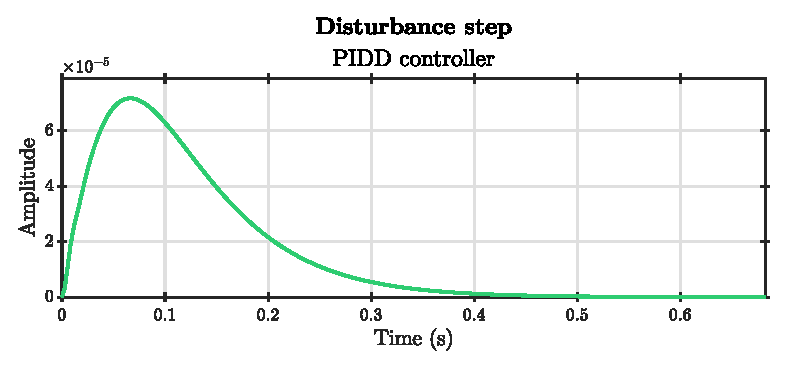
\includegraphics[]{media/q2/pidd_response.eps}
    \caption{}
    \label{fig:q2_pidd_response}
\end{figure}
\begin{figure}[ht]
    \centering
    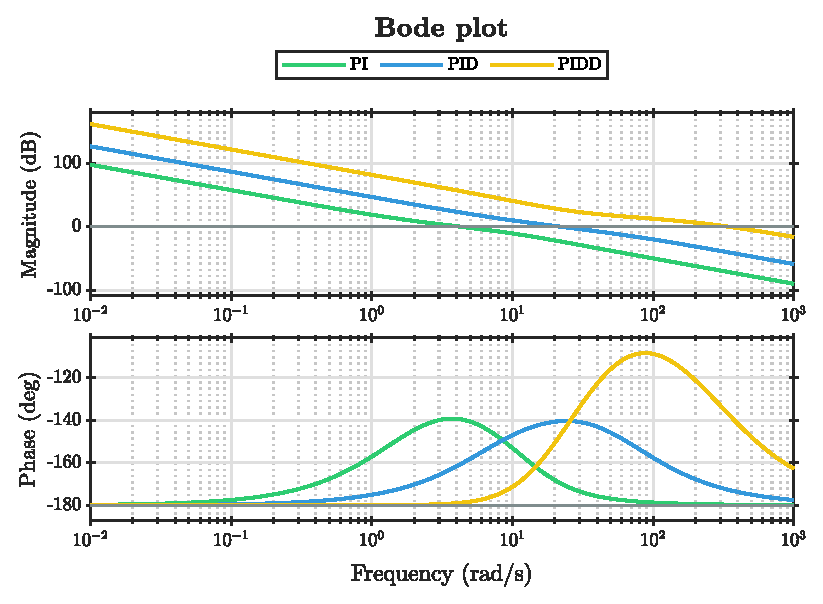
\includegraphics[]{media/q2/pi_bode_comparison.eps}
    \caption{}
    \label{fig:q2_bode_comparison}
\end{figure}